\documentclass[12pt]{article}

\usepackage{sbc-template}
\usepackage{graphicx,url}
\usepackage[utf8]{inputenc}
\usepackage[T1]{fontenc}
\usepackage[brazil]{babel}
\usepackage{booktabs,multirow,amsmath,amssymb,array,tabularx}
\usepackage{tikz}
\usetikzlibrary{positioning,arrows.meta}
\usepackage[hidelinks]{hyperref}

\sloppy
\renewcommand{\topfraction}{0.9}
\renewcommand{\bottomfraction}{0.8}
\renewcommand{\textfraction}{0.07}
\renewcommand{\floatpagefraction}{0.75}
\setcounter{topnumber}{3}
\setcounter{totalnumber}{4}

\newcommand{\ataque}[1]{\textit{#1}}

\title{Detecção de Intrusões por Anomalia em Tráfego GOOSE\\
com MLP e Random Forest: Base para um IDS Híbrido\\ com Regras Geradas por LLM}

\author{
Lucas A. Martins\inst{1},
Camilla B. Quincozes\inst{1}, Giovanni Siervo\inst{1},\\
Silvio E. Quincozes\inst{1,2}, Éderson Rosa da Silva\inst{1}
}

% [CONFIRMAR] identificadores de e-mail e se todos são @ufu.br.
\address{Universidade Federal de Uberlândia (UFU) --
Uberlândia, Brasil
\nextinstitute
Universidade Federal do Pampa (UNIPAMPA) --
Alegrete, Brasil
\email{\{lucas.martins, camillaquincozes, gsiervo, sequincozes, ersilva\}@ufu.br}}

\begin{document}

\maketitle

\begin{abstract}
The GOOSE protocol (IEC 61850) carries time-critical protection commands in
digital substations without native authentication, which exposes it to
masquerade, injection, replay and denial-of-service attacks. Specification
rules generated by Large Language Models (LLMs) are interpretable and cheap,
but only describe known behaviors. This paper builds and evaluates the anomaly
module of a hybrid intrusion detection system (IDS). We present a reproducible
notebook that lets the user choose the \textit{dataset} and the learning algorithm, and
compare a Multilayer Perceptron (MLP) with a Random Forest (RF) on the ERENO
\textit{dataset} (199,998 messages, one normal and eight attack classes). RF reached
92.41\% accuracy and 93.49\% macro-F1; the MLP reached 89.98\% and 91.09\%,
but was 26 times faster per message (0.20~ms). Both cover over 99.7\% of the
attacks that exploit missing origin authentication, missing integrity and
missing state-number validation, while missing delivery guarantees (grayhole)
and missing replay protection remain open. Finally, we fuse the models with the
LLM-generated rules from our previous work and show that selecting rules by
their false-positive rate on training data is required for the fusion to pay off.
\end{abstract}

\begin{resumo}
O protocolo GOOSE (IEC 61850) transporta comandos de proteção críticos em
subestações digitais sem autenticação nativa, o que o expõe a ataques de
falsificação, injeção, \textit{replay} e negação de serviço. Regras de
especificação geradas por Modelos de Linguagem de Grande Escala (LLMs) são
interpretáveis e baratas, mas descrevem apenas comportamentos conhecidos. Este
artigo constrói e avalia o módulo de anomalia de um sistema de detecção de
intrusão (IDS) híbrido. Apresentamos um \textit{notebook} reprodutível que
permite escolher a base de dados e o algoritmo de aprendizado, e comparamos um
\textit{Multilayer Perceptron} (MLP) com um \textit{Random Forest} (RF) no
\textit{dataset} ERENO (199.998 mensagens, uma classe normal e oito de ataque). O RF
atingiu 92,41\% de acurácia e 93,49\% de F1-macro; o MLP, 89,98\% e 91,09\%,
sendo 26 vezes mais rápido por mensagem (0,20~ms). Ambos cobrem mais de 99,7\%
dos ataques que exploram a falta de autenticação de origem, de integridade e de
validação dos contadores de estado; a falta de garantia de entrega
(\textit{grayhole}) e de proteção anti-\textit{replay} permanece em aberto.
Por fim, combinamos os modelos com as regras geradas por LLM em nosso trabalho
anterior e mostramos que selecionar as regras pela taxa de falsos positivos no
treino é necessário para que a fusão compense.
\end{resumo}

% =====================================================================
\section{Introdução}

A digitalização das subestações de energia elétrica substituiu a fiação
ponto a ponto entre equipamentos de proteção por redes Ethernet padronizadas
pela norma IEC~61850. Nesse modelo, dispositivos eletrônicos inteligentes
(IEDs) trocam eventos críticos por meio do protocolo GOOSE (\textit{Generic
Object Oriented Substation Event}), usado, por exemplo, para comandar a abertura
de disjuntores e para intertravamentos entre vãos. Mensagens GOOSE de proteção
devem chegar ao destino em até 4~ms~\cite{iec61850-8-1}. Para atender a esse
requisito, o protocolo é mapeado diretamente sobre a camada de enlace, em
\textit{multicast}, sem confirmação de entrega e, na prática, sem autenticação
nem cifragem: os mecanismos definidos pela IEC~62351-6~\cite{iec62351-6} ainda
são pouco implantados por restrições de latência e de compatibilidade de
equipamentos~\cite{quincozes2021survey,doostmohammadi2026survey}.

Essa combinação de criticidade e fragilidade torna o GOOSE um alvo conhecido.
Já foram demonstrados ataques de injeção de mensagens forjadas, de
envenenamento do contador de estado (\texttt{stNum}), de \textit{replay}, de
falsificação do publicador e de negação de
serviço~\cite{hoyos2012exploiting,kush2014poisoned,boeding2023testbed,roa2023gooseattacker}.
Um único comando falso de abertura de disjuntor pode desligar cargas,
provocar manobras indevidas ou mascarar uma falta real.

Sistemas de Detecção de Intrusão (IDSs) são, por isso, componentes essenciais
da defesa de subestações. A maior parte dos IDSs propostos para IEC~61850 é
baseada em especificação: regras derivadas da norma e do conhecimento de
especialistas descrevem o comportamento legítimo, e desvios geram
alertas~\cite{hong2014integrated,yang2017multidimensional,hong2019ieds,quincozes2021survey}.
Essa abordagem é leve e interpretável, mas escrever e manter as regras é
custoso. Em nosso trabalho apresentado no SBRC~2026~\cite{martins2026redflags},
mostramos que um LLM consegue automatizar esse processo: a partir de amostras
rotuladas, o modelo identifica \textit{red flags} comportamentais e as converte
em funções Python de detecção, executáveis em tempo real.

Regras, entretanto, reconhecem apenas aquilo que descrevem. Ataques que não
deixam uma assinatura clara em uma mensagem isolada, como o descarte seletivo
de mensagens (\ataque{grayhole}) ou o reenvio de quadros legítimos
(\ataque{random\_replay}), e variações não vistas durante a geração das regras
escapam a esse módulo. Um modelo que aprenda o perfil do tráfego complementa as
regras. Essa é a motivação de um IDS \textbf{híbrido}, em que um módulo de
assinatura (regras) e um módulo de anomalia (aprendizado de máquina) operam em
conjunto~\cite{girdhar2024sdn,yoon2025sdn}.

Este artigo constrói e avalia o módulo de anomalia desse IDS híbrido, usando
dois algoritmos clássicos e de naturezas distintas: uma rede neural
\textit{Multilayer Perceptron} (MLP) e um \textit{Random Forest} (RF). As
contribuições são:
\begin{enumerate}
\item uma ferramenta em \textit{notebook} Jupyter, reprodutível e no mesmo
  formato do artefato do SBRC~2026, que permite escolher a base de dados e o
  algoritmo, treinar, testar e gerar automaticamente matrizes de confusão,
  gráficos de detecção por classe de ataque e por falha de segurança do GOOSE;
\item uma comparação experimental entre MLP e RF no \textit{dataset}
  ERENO~\cite{quincozes2024ereno}, cobrindo qualidade de detecção, custo de
  treinamento e latência de inferência frente ao requisito de 4~ms;
\item um mapeamento entre os oito ataques do ERENO e as cinco lacunas de
  projeto do GOOSE que eles exploram, com a cobertura de cada lacuna pelos
  modelos; e
\item uma primeira avaliação da fusão entre o módulo de anomalia e as regras
  geradas por LLM, incluindo uma estratégia de seleção de regras pelo treino
  que controla os falsos positivos.
\end{enumerate}

% =====================================================================
\section{Fundamentação Teórica}\label{sec:fund}

\subsection{IEC 61850 e o protocolo GOOSE}

A IEC~61850 define um modelo de dados orientado a objetos para a automação de
subestações e o mapeia sobre diferentes protocolos de comunicação. O GOOSE é o
serviço de eventos entre IEDs. Cada publicador mantém um bloco de controle
(\texttt{gocbRef}) associado a um conjunto de dados (\texttt{datSet}) e envia
mensagens para um endereço MAC \textit{multicast}, com
\texttt{EtherType}~0x88B8. Os assinantes filtram as mensagens de interesse pelo
identificador da aplicação (\texttt{APPID}) e pelo \texttt{goID}~\cite{iec61850-8-1}.

A confiabilidade do GOOSE é obtida por retransmissão, e não por confirmação.
Quando o estado de um dado muda, o publicador incrementa o número de estado
(\texttt{stNum}), zera o número de sequência (\texttt{sqNum}) e envia a nova
mensagem em rajada, com intervalos crescentes, até voltar ao período de
\textit{heartbeat}. Enquanto o estado não muda, apenas o \texttt{sqNum} é
incrementado. Cada mensagem carrega ainda um carimbo de tempo da última
mudança de estado e o campo \texttt{timeAllowedtoLive}, que informa ao
assinante quanto tempo esperar pela próxima mensagem antes de considerar o
publicador inativo. Os assinantes aceitam, em geral, a mensagem com maior
\texttt{stNum} como a mais recente. Essa regra simples é o ponto de partida de
vários ataques.

\subsection{Falhas de segurança do GOOSE}

Do ponto de vista de segurança, o GOOSE apresenta cinco lacunas de projeto que
os ataques exploram, resumidas na Tabela~\ref{tab:falhas} e usadas ao longo
deste artigo:
\begin{description}
\item[F1 -- ausência de autenticação de origem:] qualquer estação com acesso
  ao segmento pode publicar mensagens com o MAC, o \texttt{goID} e o
  \texttt{gocbRef} de um IED legítimo, falsificando o publicador
  (\textit{masquerade});
\item[F2 -- ausência de integridade da mensagem:] não há código de autenticação
  de mensagem, de modo que quadros forjados com valores arbitrários são aceitos
  (\textit{injection});
\item[F3 -- ausência de proteção anti-\textit{replay}:] quadros legítimos
  capturados podem ser reenviados mais tarde, em ordem aleatória ou invertida,
  sem que o assinante perceba;
\item[F4 -- ausência de validação semântica de \texttt{stNum}/\texttt{sqNum}
  e de controle de taxa:] um atacante que publica um \texttt{stNum} muito alto
  faz o assinante descartar as mensagens legítimas seguintes, e rajadas em alta
  taxa sobrecarregam os IEDs~\cite{kush2014poisoned,hoyos2012exploiting};
\item[F5 -- ausência de garantia de entrega:] como não há confirmação, um nó
  comprometido no caminho pode descartar mensagens seletivamente
  (\textit{grayhole}) sem gerar erro de protocolo~\cite{kulkarni2026grayhole}.
\end{description}

\begin{table}[!htbp]
\centering
\caption{Ataques do ERENO e as falhas de segurança do GOOSE que exploram.}
\label{tab:falhas}
\small
\begin{tabular}{p{4.6cm}p{4.4cm}p{4.2cm}}
\toprule
Falha explorada & Ataque(s) no ERENO & Efeito na subestação\\
\midrule
F1 Autenticação de origem & \ataque{masquerade\_fake\_fault}, \ataque{masquerade\_fake\_normal} & falta falsa ou mascaramento de falta real\\
F2 Integridade da mensagem & \ataque{injection} & comandos com valores arbitrários\\
F3 Proteção anti-\textit{replay} & \ataque{inverse\_replay}, \ataque{random\_replay} & reaplicação de estados antigos\\
F4 Validação de \texttt{stNum}/\texttt{sqNum} e taxa & \ataque{high\_StNum}, \ataque{poisoned\_high\_rate} & bloqueio do publicador legítimo, negação de serviço\\
F5 Garantia de entrega & \ataque{grayhole} & perda seletiva de eventos\\
\bottomrule
\end{tabular}
\end{table}

A IEC~62351-6 propõe assinaturas digitais e códigos de autenticação para
mitigar F1 a F3~\cite{iec62351-6}, mas o custo computacional e a necessidade de
gestão de chaves em IEDs legados retardam sua adoção. Até que esses mecanismos estejam
disponíveis em toda a base instalada, a detecção na rede é a defesa possível.

\subsection{Sistemas de detecção de intrusão}

IDSs podem ser classificados pela fonte de dados (rede ou \textit{host}) e
pela técnica de detecção~\cite{quincozes2021survey}. IDSs por
\textbf{assinatura} ou \textbf{especificação} comparam o tráfego com padrões
conhecidos de ataque ou com o comportamento previsto pela norma: são precisos e
interpretáveis, mas não reconhecem o que não está descrito. IDSs por
\textbf{anomalia} aprendem um modelo do comportamento esperado e sinalizam
desvios: generalizam melhor, mas tendem a gerar mais falsos positivos e são
menos explicáveis. Neste trabalho usamos modelos supervisionados treinados com
tráfego normal e de ataque; a saída é tratada como anômala sempre que a classe
predita difere de \textit{normal}. Arquiteturas \textbf{híbridas} combinam as
duas técnicas para reduzir as limitações de cada uma.

\subsection{Multilayer Perceptron}

O MLP é uma rede neural de alimentação direta (\textit{feedforward}) composta por camadas de neurônios
totalmente conectadas~\cite{haykin2009neural}. A saída da camada $l$ é
$\mathbf{h}^{(l)} = \sigma(\mathbf{W}^{(l)}\mathbf{h}^{(l-1)} + \mathbf{b}^{(l)})$,
em que $\sigma$ é uma função de ativação não linear; usamos a ReLU,
$\sigma(z)=\max(0,z)$. A última camada aplica a função \textit{softmax} para
produzir uma distribuição de probabilidade sobre as $K$ classes, e os pesos são
ajustados minimizando a entropia cruzada
$\mathcal{L} = -\sum_{k=1}^{K} y_k \log \hat{y}_k + \alpha\|\mathbf{W}\|_2^2$
por retropropagação do erro~\cite{rumelhart1986learning}. Usamos o otimizador
Adam~\cite{kingma2015adam}, que adapta a taxa de aprendizado de cada parâmetro a
partir de estimativas do primeiro e do segundo momento do gradiente.

\subsection{Random Forest}

O RF é um \textit{ensemble} de árvores de decisão treinadas sobre amostras
\textit{bootstrap} do conjunto de treino~\cite{breiman2001random}. Em cada nó, a
divisão é escolhida entre um subconjunto aleatório de atributos, minimizando a
impureza de Gini $G = 1 - \sum_k p_k^2$. A classe final é obtida por votação
majoritária. A aleatoriedade na amostragem e na escolha de atributos reduz a
correlação entre as árvores e, portanto, a variância do conjunto. O RF lida bem
com atributos em escalas distintas, sem padronização, e fornece uma medida de
importância de atributos pela redução média de impureza. Seu custo de
inferência cresce com o número e a profundidade das árvores.

\subsection{Regras de detecção geradas por LLM}

No SBRC~2026~\cite{martins2026redflags}, o \textit{pipeline} recebe as médias
dos atributos do tráfego normal e de cada ataque, pede ao LLM uma lista de
\textit{red flags} justificadas pela norma e, em um segundo estágio, pede a
conversão dessas \textit{red flags} em funções Python
\texttt{rule\_<classe>\_<nome>(packet)}, que combinam ao menos dois campos e
retornam verdadeiro quando a mensagem é suspeita. O resultado é um conjunto de
22 regras para as oito classes de ataque do ERENO, avaliado em um simulador de
\textit{switch} programável. São essas regras que compõem o módulo de
assinatura do IDS híbrido proposto aqui.

% =====================================================================
\section{Trabalhos Relacionados}\label{sec:rel}

\textbf{IDSs por especificação.} Os primeiros IDSs para IEC~61850 verificam
regras derivadas da norma, como a coerência entre \texttt{stNum},
\texttt{sqNum} e o tempo entre mensagens.
Hong et al.~\cite{hong2014integrated} integram detecção baseada em
\textit{host} e em rede para GOOSE e SMV, e depois levam a detecção para dentro
dos próprios IEDs, de forma colaborativa~\cite{hong2019ieds}.
Yang et al.~\cite{yang2017multidimensional} combinam regras de acesso, de
protocolo e de comportamento. O levantamento de Quincozes et
al.~\cite{quincozes2021survey} compila essas regras e mostra que ataques de
falsificação seguem mal cobertos.

\textbf{Aprendizado de máquina supervisionado.} Bhattacharya et
al.~\cite{bhattacharya2024ml} aplicam modelos de séries temporais com
balanceamento de dados a GOOSE e SV, com taxas de acerto acima de 99\%. Senel e
Al-Hubaishi~\cite{senel2026simultaneous} avaliam 14 classificadores com mais de
50 atributos extraídos do \textit{heartbeat} GOOSE e dos endereços MAC, com
desempenho superior a 99\% para \textit{ensembles}. Yasseen e
Csatár~\cite{yasseen2026optimal,yasseen2025ml} mostram que a duração e os
tempos entre chegadas são os atributos mais discriminantes, e Eynawi et
al.~\cite{eynawi2024feature} chegam a conclusão semelhante para SV e MMS.
Kulkarni et al.~\cite{kulkarni2026grayhole} modelam ataques \ataque{grayhole}
no ERENO e obtêm F1 de 90,7\% com árvore J48, em um conjunto pequeno de mil
amostras.

\textbf{Aprendizado profundo e não supervisionado.} Fernando et
al.~\cite{fernando2025spoofing} combinam DNN, LSTM e \textit{autoencoders} para detectar
falsificação. Lozano-Paredes et al.~\cite{lozano2026explainable} propõem
\textit{autoencoders} assimétricos que separam visões semântica e temporal, com
explicabilidade por erro de reconstrução. Goyel et
al.~\cite{goyel2026transformer} usam \textit{transformers} com ajuste de
distribuição para definir limiares, e Jay et
al.~\cite{jay2022unsupervised,jay2025iidm} combinam técnicas estatísticas e de
\textit{ensemble} não supervisionado. Elbez et al.~\cite{elbez2024eda4gnet}
modelam matematicamente o tráfego GOOSE para detecção precoce de DoS.

\textbf{Trabalhos no ERENO.} O ERENO~\cite{quincozes2022ereno,quincozes2024ereno}
é um gerador de tráfego IEC~61850 sintético e realista que produz conjuntos com
oito casos de uso. Moore~\cite{moore2026anomaly} compara, no ERENO, um RF
supervisionado com \textit{autoencoders} recorrentes: o RF obtém o maior F1 (0,95), mas
não cumpre o limite de 4~ms, com 21,8~ms por predição. O GOOSEIDRS de Alberto et
al.~\cite{alberto2026gooseidrs} usa LightGBM com atributos centrados em
\texttt{stNum}/\texttt{sqNum} e responde automaticamente a ataques de
falsificação.

\textbf{LLMs para segurança de subestações.} Zaboli et
al.~\cite{zaboli2024chatgpt,zaboli2025genai} usam LLMs com humano no ciclo (\textit{human-in-the-loop}) e
depois sistemas de diálogo orientados a tarefas para detectar anomalias em GOOSE
e SV. Danso et al.~\cite{danso2025llm} alimentam o ChatGPT com rastros GOOSE.
Manzoor et al.~\cite{manzoor2024zeroday} exploram aprendizado em contexto para
ataques de dia zero, e Li et al.~\cite{li2025racl} combinam aprendizado
contrastivo e LLM para gerar relatórios. Na geração de regras, o GenTI de Hadi et
al.~\cite{hadi2026genti} produz regras Snort/Suricata a partir de
inteligência de ameaças, e o CritBench de Keppler et al.~\cite{keppler2026critbench}
avalia agentes LLM em tarefas de subestação. 

\textbf{Arquiteturas híbridas.} Girdhar et al.~\cite{girdhar2024sdn} e Yoon et
al.~\cite{yoon2025sdn} combinam verificação de regras e aprendizado profundo em
arquiteturas SDN, isolando portas de IEDs comprometidos. Em ambos, as regras são
escritas manualmente. A Tabela~\ref{tab:rel} posiciona este trabalho. Até onde
sabemos, ele é o primeiro a combinar um módulo de anomalia com regras de
assinatura \emph{geradas por LLM} para GOOSE, e a avaliar o efeito da fusão
sobre os falsos positivos.

\begin{table}[!htbp]
\centering
\caption{Comparação com trabalhos relacionados.}
\label{tab:rel}
\small
\begin{tabular}{lcccccc}
\toprule
Trabalho & \textit{Dataset} & Supervis. & Regras & Regras LLM & Latência & Híbrido\\
\midrule
\cite{hong2014integrated,yang2017multidimensional} & próprio & -- & \checkmark & -- & -- & --\\
\cite{bhattacharya2024ml,senel2026simultaneous} & públicos & \checkmark & -- & -- & -- & --\\
\cite{lozano2026explainable,goyel2026transformer} & próprio/púb. & -- & -- & -- & -- & --\\
\cite{moore2026anomaly} & ERENO & \checkmark & -- & -- & \checkmark & --\\
\cite{alberto2026gooseidrs} & próprio & \checkmark & -- & -- & \checkmark & --\\
\cite{girdhar2024sdn,yoon2025sdn} & próprio/púb. & \checkmark & \checkmark & -- & -- & \checkmark\\
\cite{martins2026redflags} & ERENO & -- & \checkmark & \checkmark & \checkmark & --\\
\textbf{Este trabalho} & ERENO & \checkmark & \checkmark & \checkmark & \checkmark & \checkmark\\
\bottomrule
\end{tabular}
\end{table}

% =====================================================================
\section{Proposta: IDS Híbrido para GOOSE}\label{sec:prop}

A Figura~\ref{fig:arq} apresenta a arquitetura proposta. O tráfego GOOSE do
barramento de estação é copiado por espelhamento de porta ou TAP, de modo que o
IDS não insere latência no caminho das mensagens de proteção. Um extrator
monta, para cada mensagem, o vetor de atributos do cabeçalho GOOSE, os
atributos derivados em relação à mensagem anterior do mesmo publicador e,
quando disponíveis, as medidas elétricas associadas.

\begin{figure}[!htbp]
\centering
\resizebox{\linewidth}{!}{% Diagrama da arquitetura do IDS hibrido (TikZ) -- incluido via % Diagrama da arquitetura do IDS hibrido (TikZ) -- incluido via % Diagrama da arquitetura do IDS hibrido (TikZ) -- incluido via \input{arquitetura}
\begin{tikzpicture}[
  font=\footnotesize, >=Stealth, node distance=4mm and 6mm,
  box/.style={draw=black!60, rounded corners=2pt, align=center, minimum height=9mm, inner sep=3pt, fill=white},
  sig/.style={box, fill=green!8}, ano/.style={box, fill=blue!8}, dec/.style={box, fill=violet!10},
  lbl/.style={font=\scriptsize\itshape, text=black!65}]
  \node[box, minimum width=22mm] (in) {Tr\'afego GOOSE\\(espelhamento / TAP)};
  \node[box, right=of in, minimum width=22mm] (pre) {Extra\c{c}\~ao de\\atributos};
  \node[sig, above right=3mm and 8mm of pre, minimum width=36mm] (sig)
       {\textbf{M\'odulo de assinatura}\\regras geradas por LLM\\(SBRC 2026)};
  \node[ano, below right=3mm and 8mm of pre, minimum width=36mm] (ano)
       {\textbf{M\'odulo de anomalia}\\MLP ou Random Forest\\(este trabalho)};
  \node[dec, anchor=west, minimum width=24mm] (fus) at ([xshift=12mm]sig.east |- pre.east) {\textbf{Fus\~ao}\\OU seletivo};
  \node[box, right=of fus, minimum width=20mm] (out) {Alerta /\\bloqueio};
  \draw[->] (in) -- (pre);
  \draw[->] (pre.east) -- ++(3mm,0) |- (sig.west);
  \draw[->] (pre.east) -- ++(3mm,0) |- (ano.west);
  \draw[->] (sig.east) -- ++(5mm,0) |- (fus.west);
  \draw[->] (ano.east) -- ++(5mm,0) |- (fus.west);
  \draw[->] (fus) -- (out);
  \node[lbl, above=0.5mm of sig] {ataques conhecidos, interpret\'avel, plano de dados (P4)};
  \node[lbl, below=0.5mm of ano] {desvios do comportamento normal aprendido};
\end{tikzpicture}

\begin{tikzpicture}[
  font=\footnotesize, >=Stealth, node distance=4mm and 6mm,
  box/.style={draw=black!60, rounded corners=2pt, align=center, minimum height=9mm, inner sep=3pt, fill=white},
  sig/.style={box, fill=green!8}, ano/.style={box, fill=blue!8}, dec/.style={box, fill=violet!10},
  lbl/.style={font=\scriptsize\itshape, text=black!65}]
  \node[box, minimum width=22mm] (in) {Tr\'afego GOOSE\\(espelhamento / TAP)};
  \node[box, right=of in, minimum width=22mm] (pre) {Extra\c{c}\~ao de\\atributos};
  \node[sig, above right=3mm and 8mm of pre, minimum width=36mm] (sig)
       {\textbf{M\'odulo de assinatura}\\regras geradas por LLM\\(SBRC 2026)};
  \node[ano, below right=3mm and 8mm of pre, minimum width=36mm] (ano)
       {\textbf{M\'odulo de anomalia}\\MLP ou Random Forest\\(este trabalho)};
  \node[dec, anchor=west, minimum width=24mm] (fus) at ([xshift=12mm]sig.east |- pre.east) {\textbf{Fus\~ao}\\OU seletivo};
  \node[box, right=of fus, minimum width=20mm] (out) {Alerta /\\bloqueio};
  \draw[->] (in) -- (pre);
  \draw[->] (pre.east) -- ++(3mm,0) |- (sig.west);
  \draw[->] (pre.east) -- ++(3mm,0) |- (ano.west);
  \draw[->] (sig.east) -- ++(5mm,0) |- (fus.west);
  \draw[->] (ano.east) -- ++(5mm,0) |- (fus.west);
  \draw[->] (fus) -- (out);
  \node[lbl, above=0.5mm of sig] {ataques conhecidos, interpret\'avel, plano de dados (P4)};
  \node[lbl, below=0.5mm of ano] {desvios do comportamento normal aprendido};
\end{tikzpicture}

\begin{tikzpicture}[
  font=\footnotesize, >=Stealth, node distance=4mm and 6mm,
  box/.style={draw=black!60, rounded corners=2pt, align=center, minimum height=9mm, inner sep=3pt, fill=white},
  sig/.style={box, fill=green!8}, ano/.style={box, fill=blue!8}, dec/.style={box, fill=violet!10},
  lbl/.style={font=\scriptsize\itshape, text=black!65}]
  \node[box, minimum width=22mm] (in) {Tr\'afego GOOSE\\(espelhamento / TAP)};
  \node[box, right=of in, minimum width=22mm] (pre) {Extra\c{c}\~ao de\\atributos};
  \node[sig, above right=3mm and 8mm of pre, minimum width=36mm] (sig)
       {\textbf{M\'odulo de assinatura}\\regras geradas por LLM\\(SBRC 2026)};
  \node[ano, below right=3mm and 8mm of pre, minimum width=36mm] (ano)
       {\textbf{M\'odulo de anomalia}\\MLP ou Random Forest\\(este trabalho)};
  \node[dec, anchor=west, minimum width=24mm] (fus) at ([xshift=12mm]sig.east |- pre.east) {\textbf{Fus\~ao}\\OU seletivo};
  \node[box, right=of fus, minimum width=20mm] (out) {Alerta /\\bloqueio};
  \draw[->] (in) -- (pre);
  \draw[->] (pre.east) -- ++(3mm,0) |- (sig.west);
  \draw[->] (pre.east) -- ++(3mm,0) |- (ano.west);
  \draw[->] (sig.east) -- ++(5mm,0) |- (fus.west);
  \draw[->] (ano.east) -- ++(5mm,0) |- (fus.west);
  \draw[->] (fus) -- (out);
  \node[lbl, above=0.5mm of sig] {ataques conhecidos, interpret\'avel, plano de dados (P4)};
  \node[lbl, below=0.5mm of ano] {desvios do comportamento normal aprendido};
\end{tikzpicture}
}
\caption{Arquitetura do IDS híbrido proposto.}
\label{fig:arq}
\end{figure}

\textbf{Módulo de assinatura.} Aplica as regras geradas pelo \textit{pipeline}
do SBRC~2026. Por serem compostas apenas de comparações entre campos, as regras
podem ser traduzidas para tabelas \textit{match-action} e executadas em planos
de dados programáveis em P4~\cite{bosshart2014p4,xavier2021programmable,fida2026pdpsurvey},
na taxa de linha. Cada disparo identifica a \textit{red flag} violada, o que facilita explicar o alerta.

\textbf{Módulo de anomalia.} É o foco deste artigo. Um classificador (MLP ou RF)
recebe o vetor de atributos e prediz uma das nove classes. Qualquer predição
diferente de \textit{normal} é tratada como anômala. A predição multiclasse é
mantida porque indica a falha de segurança explorada (Tabela~\ref{tab:falhas}).

\textbf{Fusão.} Combina os dois módulos. A forma mais simples é o OU lógico:
um alerta é emitido se o modelo ou alguma regra sinalizar a mensagem. Como os
falsos positivos dos dois módulos se somam, propomos a \textbf{fusão seletiva}:
apenas regras cujo disparo em tráfego normal, medido no conjunto de treino,
seja menor ou igual a um limiar $\tau$ participam da fusão. Formalmente, sendo
$\mathcal{R}$ o conjunto de regras, $\mathcal{N}_{tr}$ as mensagens normais de
treino e $r(x)\in\{0,1\}$ o disparo da regra $r$ na mensagem $x$,
\begin{equation}
\mathcal{R}_\tau = \Big\{ r \in \mathcal{R} : \frac{1}{|\mathcal{N}_{tr}|}\sum_{x\in\mathcal{N}_{tr}} r(x) \le \tau \;\wedge\; \exists\,x \in \mathcal{A}_{tr}: r(x)=1 \Big\},
\end{equation}
em que $\mathcal{A}_{tr}$ são as mensagens de ataque de treino, e o alerta final é
$\hat{y}(x) = \mathbb{1}[f(x)\neq\textit{normal}] \lor \bigvee_{r\in\mathcal{R}_\tau} r(x)$,
com $f$ o classificador. Usamos $\tau = 0{,}5\%$. A seleção usa apenas o
treino, de modo que o conjunto de teste não influencia quais regras entram.

% =====================================================================
\section{Metodologia}\label{sec:met}

\subsection{Dataset e limpeza}

Utilizamos o arquivo ERENO-2.0-100K, o mesmo do artefato do
SBRC~2026~\cite{martins2026redflags}, gerado pelo
ERENO~\cite{quincozes2024ereno}. O arquivo tem 200.052 linhas e 52 colunas; 54
dessas linhas são cabeçalhos ARFF (\texttt{@relation}, \texttt{@attribute})
concatenados no meio do arquivo e foram removidas, restando 199.998 mensagens.
A Figura~\ref{fig:dist} mostra a distribuição: 39.999 mensagens normais e cerca
de 20 mil para cada ataque, ou seja, 80\% de tráfego de ataque.

\begin{figure}[!htbp]
\centering
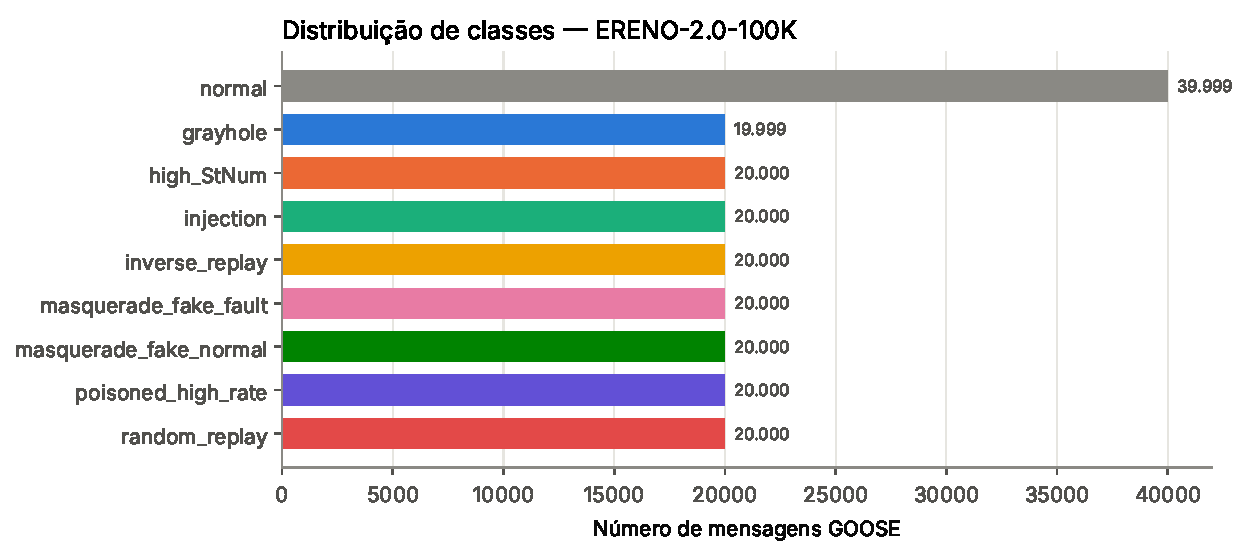
\includegraphics[width=0.62\linewidth]{figuras/fig01_distribuicao_classes.pdf}
\caption{Distribuição de classes no ERENO-2.0-100K após a limpeza.}
\label{fig:dist}
\end{figure}

Onze colunas categóricas (\texttt{ethSrc}, \texttt{ethDst}, \texttt{ethType},
\texttt{gooseAppid}, \texttt{TPID}, \texttt{gocbRef}, \texttt{datSet},
\texttt{goID}, \texttt{test}, \texttt{ndsCom} e \texttt{protocol}) têm valor
único em todo o arquivo e foram descartadas. Os carimbos de tempo absolutos
\texttt{Time}, \texttt{t} e \texttt{GooseTimestamp} também foram removidos: como
o ERENO gera cada cenário em sequência, esses campos poderiam permitir que o
modelo aprendesse a ordem da simulação, e não o comportamento do ataque. A
Tabela~\ref{tab:atrib} lista os 37 atributos mantidos.

\begin{table}[!htbp]
\centering
\caption{Atributos utilizados (37).}
\label{tab:atrib}
\small
\begin{tabularx}{\linewidth}{lX}
\toprule
Grupo & Atributos\\
\midrule
Cabeçalho GOOSE (9) & \texttt{SqNum}, \texttt{StNum}, \texttt{cbStatus}, \texttt{frameLen}, \texttt{gooseTimeAllowedtoLive}, \texttt{gooseLen}, \texttt{confRev}, \texttt{numDatSetEntries}, \texttt{APDUSize}\\
Derivados (10) & \texttt{stDiff}, \texttt{sqDiff}, \texttt{gooseLengthDiff}, \texttt{cbStatusDiff}, \texttt{apduSizeDiff}, \texttt{frameLengthDiff}, \texttt{timestampDiff}, \texttt{tDiff}, \texttt{timeFromLastChange}, \texttt{delay}\\
Elétricos (18) & correntes e tensões instantâneas das fases A, B e C (\texttt{isb*}, \texttt{vsb*}), seus valores RMS e somas de área trapezoidal\\
\bottomrule
\end{tabularx}
\end{table}

O \textit{notebook} também oferece o conjunto \texttt{protocolo}, com apenas os
19 atributos de cabeçalho e derivados, que são os campos disponíveis para as
regras do SBRC~2026 e os mais simples de extrair em um \textit{switch}.

\subsection{Divisão e pré-processamento}

O conjunto foi dividido de forma estratificada em 70\% para treino (139.998
mensagens) e 30\% para teste (60.000 mensagens), com semente fixa
(\texttt{random\_state}=42). Para o MLP, os atributos foram padronizados
($z$-score) com média e desvio-padrão estimados apenas no treino. O RF usa os
valores originais. 

\subsection{Modelos e hiperparâmetros}

A Tabela~\ref{tab:hiper} resume a configuração. O \textit{early stopping} interrompe o treino quando a
acurácia em 10\% do treino separados para validação não melhora por 10 épocas
consecutivas. O RF usa 100 árvores sem limite de profundidade. Ambos foram
implementados em scikit-learn~\cite{pedregosa2011scikit}. Não houve busca de
hiperparâmetros: o objetivo é estabelecer uma linha de base reprodutível para
o módulo de anomalia.

\begin{table}[!htbp]
\centering
\caption{Hiperparâmetros.}
\label{tab:hiper}
\small
\begin{tabular}{ll}
\toprule
MLP & Random Forest\\
\midrule
camadas ocultas: (128, 64), ReLU & árvores: 100\\
otimizador: Adam, taxa $10^{-3}$ & critério: Gini\\
regularização L2: $\alpha = 10^{-4}$ & profundidade máxima: ilimitada\\
lote: 256; épocas máx.: 200 & mínimo por folha: 1\\
\textit{early stopping}: 10\% validação, paciência 10 & atributos por divisão: $\sqrt{37}$\\
entrada padronizada ($z$-score) & entrada original\\
\bottomrule
\end{tabular}
\end{table}

\subsection{Métricas}

Na tarefa multiclasse (9 classes), reportamos acurácia e precisão,
\textit{recall} e F1 em média macro, que dá o mesmo peso a todas as classes.
Na visão binária (normal $\times$ ataque), que corresponde ao papel de detector
de anomalia, reportamos a taxa de verdadeiros positivos
$\mathrm{TPR}=\mathrm{VP}/(\mathrm{VP}+\mathrm{FN})$, a taxa de falsos
positivos $\mathrm{FPR}=\mathrm{FP}/(\mathrm{FP}+\mathrm{VN})$, a precisão e o
F1. A latência foi medida de duas formas: em lote, dividindo o tempo de
predição das 60.000 mensagens pelo total; e unitária, como a média de 500
predições de uma mensagem por vez, com uma única \textit{thread}, que é o cenário
de um IDS que decide mensagem a mensagem.

\subsection{Ferramenta e ambiente}

O \textit{notebook} \texttt{IDS\_GOOSE\_Anomalia\_MLP\_RF.ipynb} segue a
organização do artefato do SBRC~2026, com seções numeradas, saídas
exportadas e sementes fixas. A Tabela~\ref{tab:nb} descreve suas seções. Na
primeira célula, o usuário define o \textit{dataset} (\texttt{DATASET}, uma chave do
dicionário \texttt{DATASETS}, apontando para \texttt{dataset/}) e o algoritmo
(\texttt{ALGORITMO} igual a \texttt{"MLP"}, \texttt{"RF"} ou \texttt{"AMBOS"}),
ou faz a escolha por menus interativos. Todos os gráficos são salvos em PNG e
PDF em \texttt{resultados/figuras}, e as tabelas, em CSV em
\texttt{resultados/dados}, junto com um arquivo JSON de metadados do
experimento. Os experimentos foram executados em um contêiner Linux com 2 vCPUs
e 7~GB de RAM, Python~3.13 e scikit-learn~1.9; a execução completa, com os dois
algoritmos e a fusão, leva cerca de 2,5 minutos.

\begin{table}[!htbp]
\centering
\caption{Seções do \textit{notebook}.}
\label{tab:nb}
\small
\begin{tabularx}{\linewidth}{lX}
\toprule
Seção & Conteúdo\\
\midrule
§1 Configuração & escolha do \textit{dataset}, do algoritmo, do conjunto de atributos e dos hiperparâmetros\\
§2--4 Preparação & \textit{setup}, ingestão e limpeza do ERENO, divisão e padronização\\
§5 Treinamento & treino do MLP e/ou RF, curvas de perda e validação do MLP\\
§6 Teste do IDS & métricas multiclasse e binárias, latência em lote e unitária\\
§7 Matrizes & matrizes de confusão multiclasse e binária por modelo\\
§8 Detecção por classe & tráfego anômalo real $\times$ detectado para cada ataque\\
§9 Falhas GOOSE & detecções agregadas pelas falhas F1--F5\\
§10 Comparativo & MLP $\times$ RF, F1 por classe, importância e ablação de atributos\\
§11 Híbrido & aplicação das regras LLM, seleção pelo treino e fusões\\
§12 Exportação & CSVs, figuras e metadados\\
\bottomrule
\end{tabularx}
\end{table}

% =====================================================================
\section{Resultados}\label{sec:res}

\subsection{Treinamento}

O RF foi treinado em 24~s. O MLP levou 64~s e foi interrompido pelo
\textit{early stopping} após 80 épocas. A Figura~\ref{fig:curva} mostra que a
perda cai rapidamente nas primeiras 20 épocas e que a acurácia de validação se
estabiliza perto de 90\%, sem sinal de sobreajuste.

\begin{figure}[!htbp]
\centering
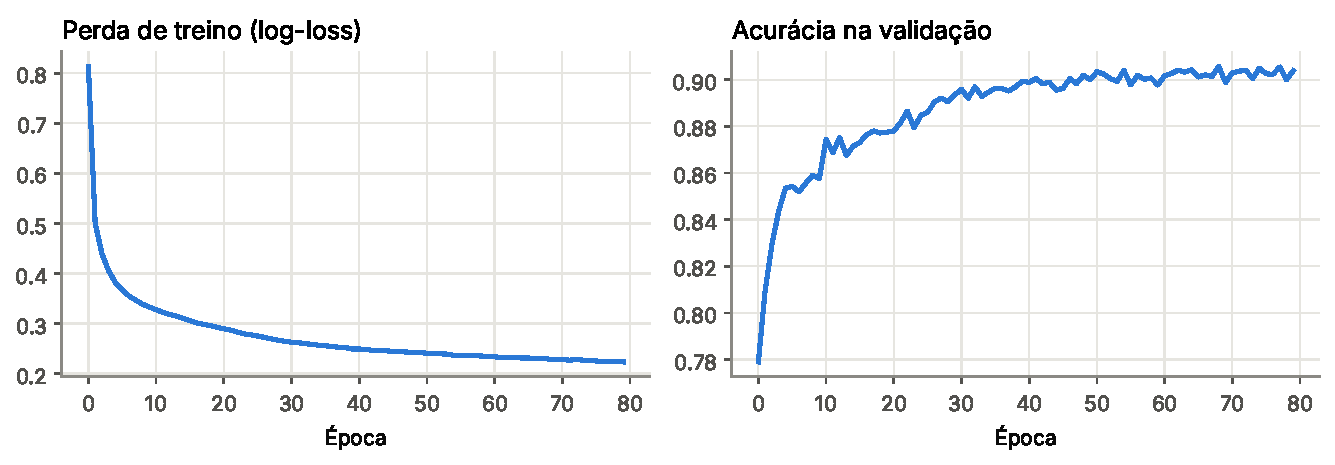
\includegraphics[width=0.78\linewidth]{figuras/fig02_mlp_curva_treino.pdf}
\caption{Curvas de treinamento do MLP.}
\label{fig:curva}
\end{figure}

\subsection{Desempenho global}

A Tabela~\ref{tab:res} e a Figura~\ref{fig:comp} comparam os dois modelos. O RF
é superior em todas as métricas de qualidade: 92,41\% de acurácia e 93,49\% de
F1-macro, contra 89,98\% e 91,09\% do MLP. Na visão binária, a diferença é
menor: o RF detecta 93,95\% das mensagens de ataque com 13,11\% de falsos
positivos, e o MLP, 93,53\% com 16,12\%.

\begin{table}[!htbp]
\centering
\caption{Desempenho no conjunto de teste (60.000 mensagens). Valores em \%.}
\label{tab:res}
\small
\begin{tabular}{lcccccccc}
\toprule
& \multicolumn{4}{c}{9 classes (macro)} & \multicolumn{4}{c}{Normal $\times$ ataque}\\
\cmidrule(lr){2-5}\cmidrule(lr){6-9}
Modelo & Acur. & Prec. & Rec. & F1 & TPR & FPR & Prec. & F1\\
\midrule
MLP & 89,98 & 91,84 & 90,66 & 91,09 & 93,53 & 16,12 & 95,87 & 94,68\\
RF  & \textbf{92,41} & \textbf{94,11} & \textbf{93,03} & \textbf{93,49} & \textbf{93,95} & \textbf{13,11} & \textbf{96,63} & \textbf{95,27}\\
\bottomrule
\end{tabular}
\end{table}

\begin{figure}[!htbp]
\centering
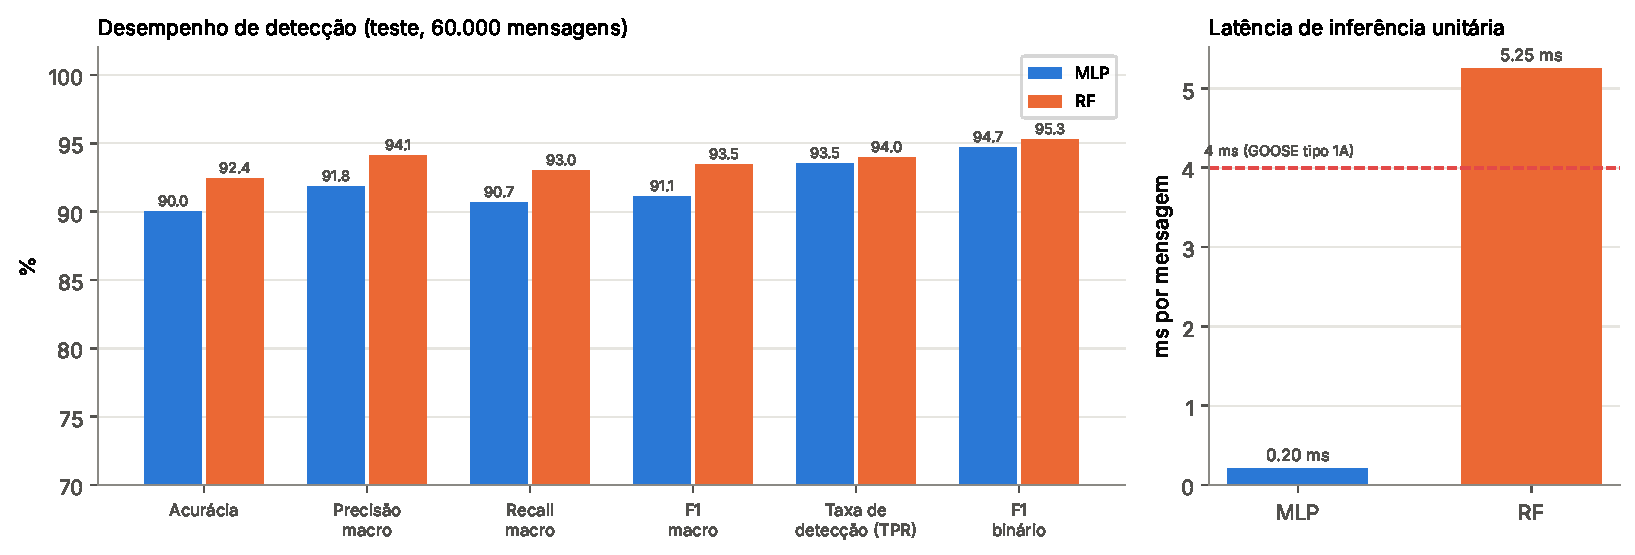
\includegraphics[width=\linewidth]{figuras/fig07_comparativo_mlp_rf.pdf}
\caption{Comparativo MLP $\times$ RF: métricas de detecção (esquerda) e
latência de inferência unitária frente ao limite de 4~ms (direita).}
\label{fig:comp}
\end{figure}

A latência inverte a vantagem. Na inferência unitária, o MLP leva 0,20~ms por
mensagem e o RF, 5,3~ms, 26 vezes mais e acima do limite de 4~ms das mensagens
GOOSE de proteção. Em lote, os custos caem para 2,7~$\mu$s (MLP) e 8,7~$\mu$s
(RF) por mensagem. A diferença indica que a latência unitária do RF é dominada pela sobrecarga
de percorrer 100 árvores para uma única amostra em Python.
Em três execuções, a latência unitária variou de 0,18 a 0,20~ms (MLP) e de 5,3 a 7,1~ms (RF), sempre acima do limite no RF, o que é coerente com Moore~\cite{moore2026anomaly} (21,8~ms).

\subsection{Matrizes de confusão}

A Figura~\ref{fig:cm-mlp} mostra as matrizes de confusão
normalizadas por classe real. Nos dois modelos, seis classes de ataque têm
acerto próximo de 100\%, e os erros se concentram em dois pares.

\begin{figure}[!htbp]
\centering
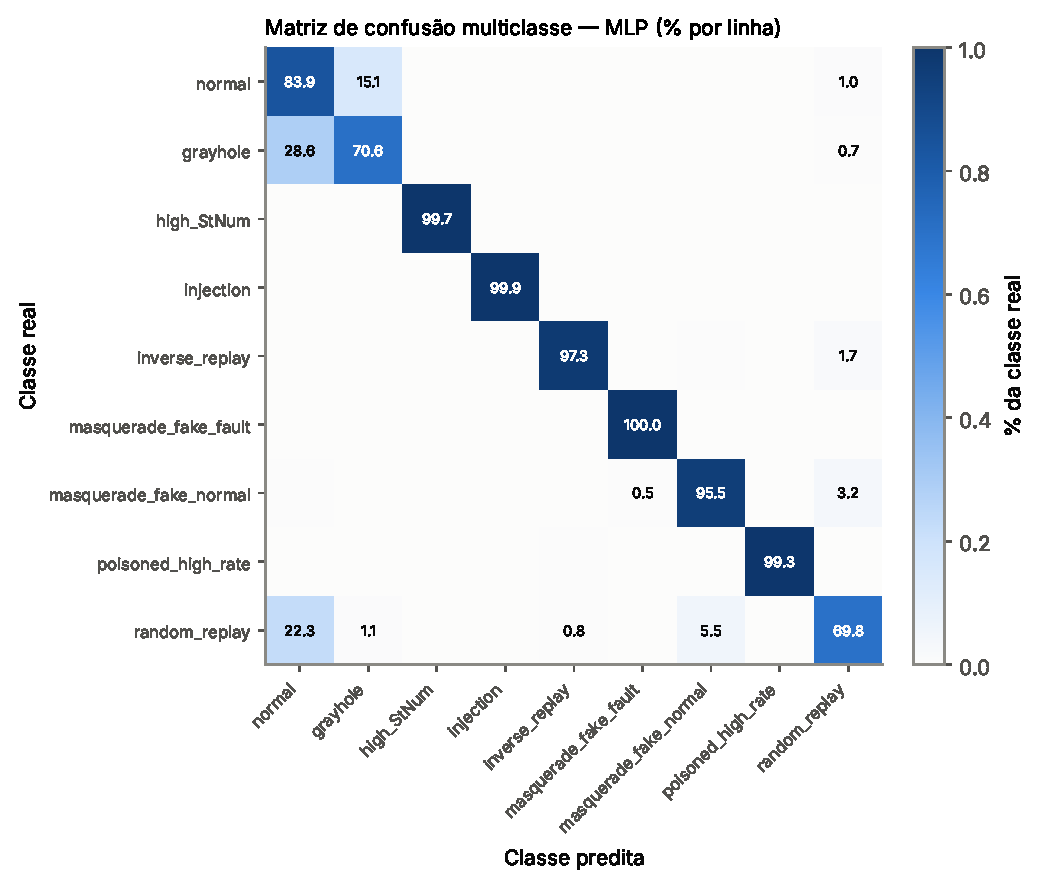
\includegraphics[width=0.495\linewidth]{figuras/fig03_cm_multiclasse_MLP.pdf}\hfill
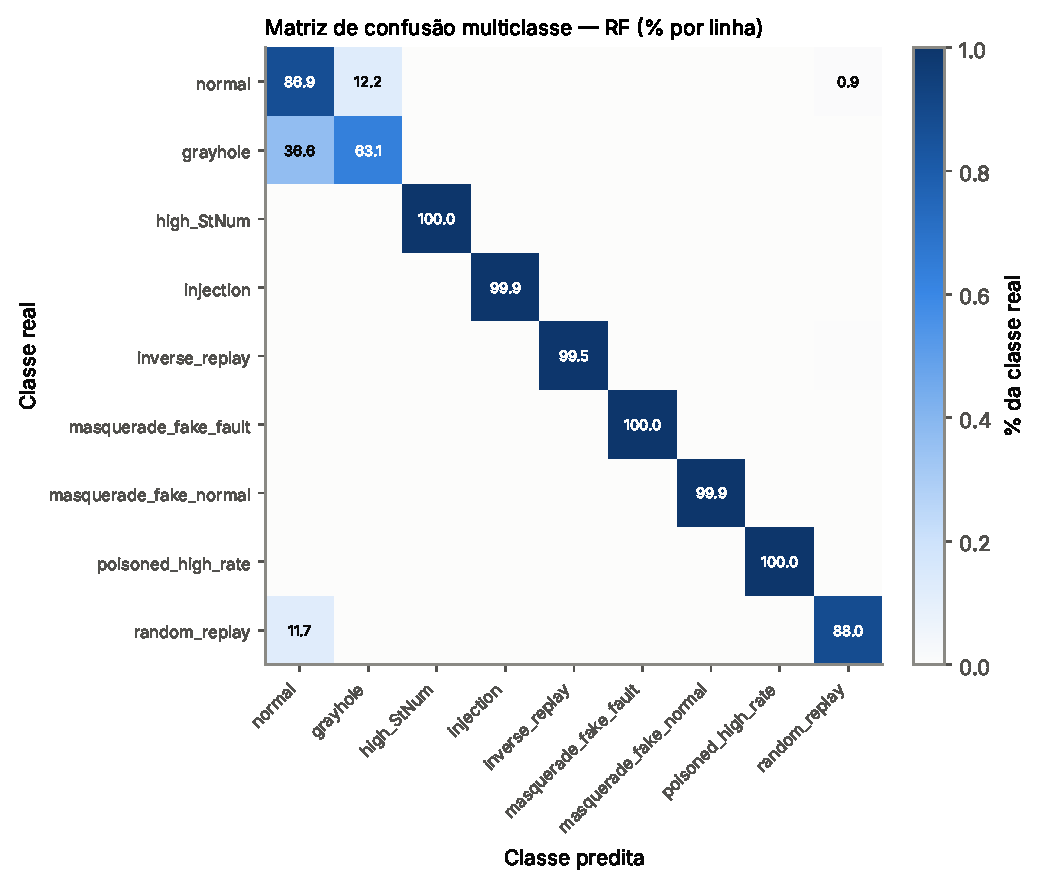
\includegraphics[width=0.495\linewidth]{figuras/fig03_cm_multiclasse_RF.pdf}
\caption{Matrizes de confusão multiclasse (\% por classe real): MLP à esquerda (a) e Random Forest à direita (b).}
\label{fig:cm-mlp}\label{fig:cm-rf}
\end{figure}

O primeiro par é \ataque{grayhole} $\leftrightarrow$ \textit{normal}. No RF,
36,6\% das mensagens de \ataque{grayhole} são classificadas como normais e
12,2\% das normais como \ataque{grayhole}; no MLP, 28,6\% e 15,1\%. Esses
erros respondem pela maior parte dos falsos positivos da visão binária. O
segundo par é \ataque{random\_replay} $\to$ \textit{normal}: 11,7\% no RF e
22,3\% no MLP. O MLP comete ainda um erro que o RF não comete:
3,2\% das mensagens de \ataque{masquerade\_fake\_normal} são classificadas como
\ataque{random\_replay}. As matrizes binárias
(Figura~\ref{fig:cm-bin}) resumem o efeito na detecção.

\begin{figure}[!htbp]
\centering
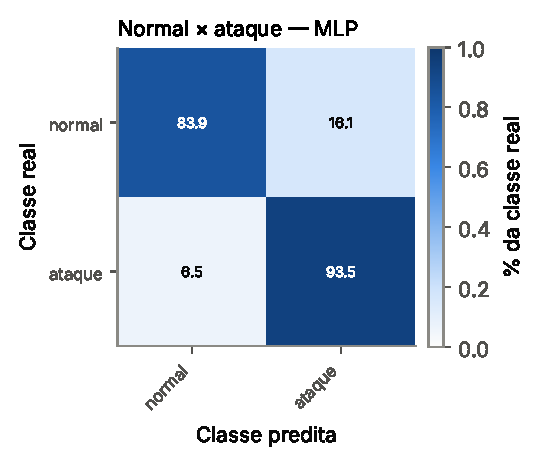
\includegraphics[width=0.34\linewidth]{figuras/fig04_cm_binaria_MLP.pdf}\hspace{1cm}
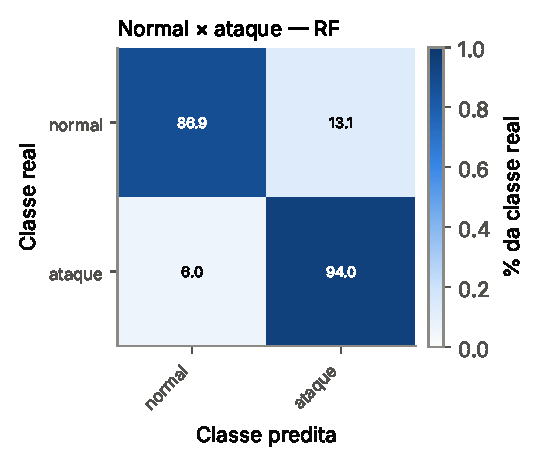
\includegraphics[width=0.34\linewidth]{figuras/fig04_cm_binaria_RF.pdf}
\caption{Matrizes de confusão binárias (normal $\times$ ataque): MLP à
esquerda, RF à direita.}
\label{fig:cm-bin}
\end{figure}

\subsection{Detecção por classe de ataque}

A Figura~\ref{fig:det} compara, para cada ataque, o total de mensagens no
teste, as mensagens sinalizadas como anômalas e as atribuídas ao ataque
correto, e a Tabela~\ref{tab:f1} traz o F1 por classe. Os ataques
\ataque{high\_StNum}, \ataque{injection}, \ataque{masquerade\_fake\_fault} e
\ataque{poisoned\_high\_rate} são detectados em 99,98\% a 100\% dos casos pelos
dois modelos. A maior diferença entre eles está no \ataque{random\_replay}: o RF
sinaliza 88,27\% das mensagens e o MLP, 77,68\% (F1 de 92,36\% contra 78,59\%).
O \ataque{grayhole} é o único ataque em que o MLP supera o RF em detecção
(71,38\% contra 63,42\%), embora com F1 semelhante, já que o MLP também gera
mais falsos positivos nessa classe.

\begin{figure}[!htbp]
\centering
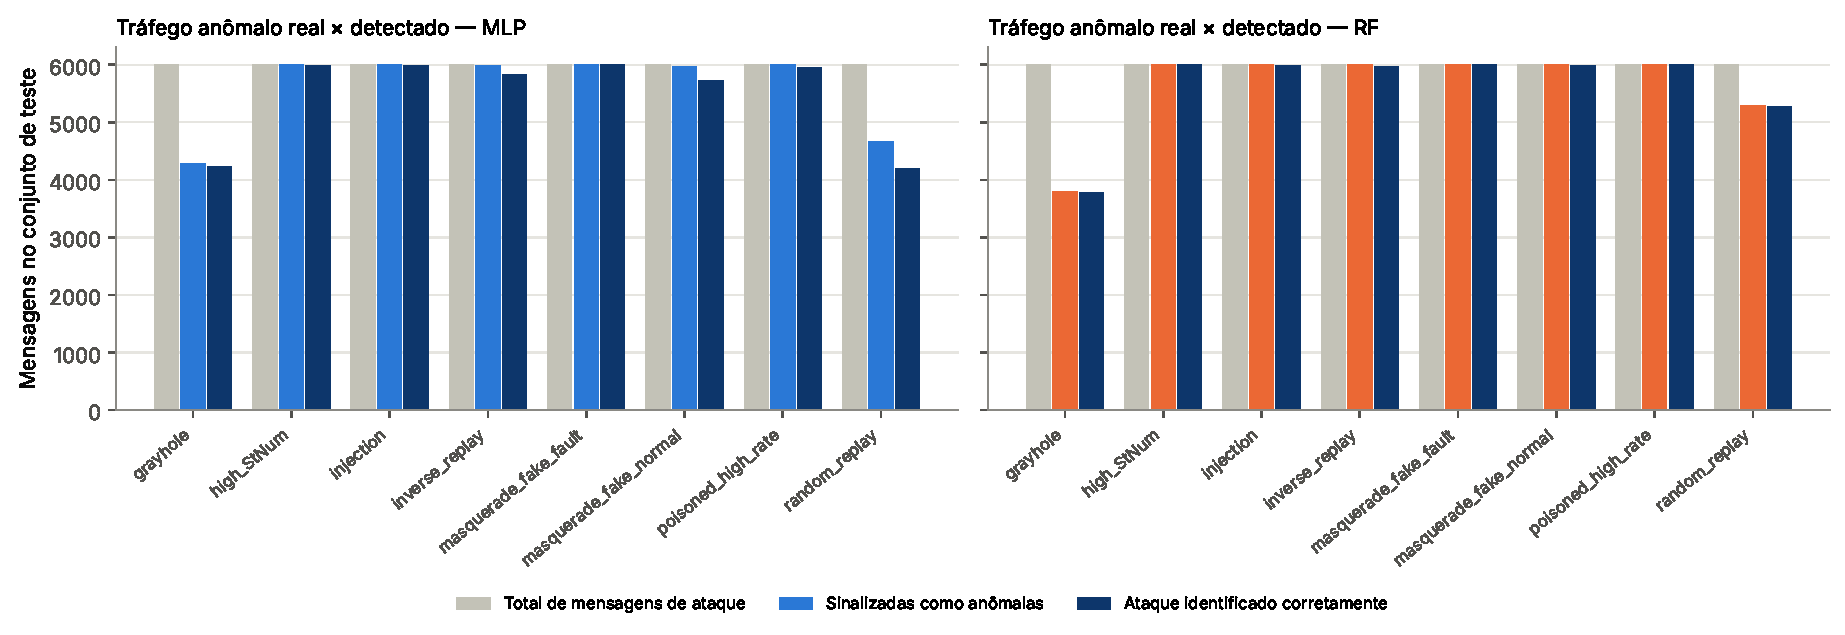
\includegraphics[width=0.92\linewidth]{figuras/fig05_deteccao_por_classe.pdf}
\caption{Tráfego anômalo real $\times$ detectado por classe de ataque.}
\label{fig:det}
\end{figure}

\begin{table}[!htbp]
\centering
\caption{F1-score por classe e taxa de detecção (sinalização como anômala), em \%.}
\label{tab:f1}
\small
\begin{tabular}{lcccc}
\toprule
& \multicolumn{2}{c}{F1} & \multicolumn{2}{c}{Detecção}\\
\cmidrule(lr){2-3}\cmidrule(lr){4-5}
Classe & MLP & RF & MLP & RF\\
\midrule
normal                  & 79,97 & 82,33 & -- & --\\
grayhole                & 69,85 & 67,27 & 71,38 & 63,42\\
high\_StNum             & 99,82 & 99,98 & 99,98 & 100,00\\
injection               & 99,92 & 99,94 & 99,98 & 99,98\\
inverse\_replay         & 97,89 & 99,72 & 99,65 & 99,97\\
masquerade\_fake\_fault & 99,40 & 99,96 & 100,00 & 100,00\\
masquerade\_fake\_normal& 94,76 & 99,81 & 99,53 & 99,97\\
poisoned\_high\_rate    & 99,55 & 99,99 & 100,00 & 100,00\\
random\_replay          & 78,59 & 92,36 & 77,68 & 88,27\\
\bottomrule
\end{tabular}
\end{table}

\subsection{Falhas de segurança do GOOSE}

A Figura~\ref{fig:falhas} agrega as detecções pelas falhas F1--F5 da
Tabela~\ref{tab:falhas}. A falta de autenticação de origem (F1), de integridade
(F2) e de validação de \texttt{stNum}/\texttt{sqNum} (F4) é coberta em mais de
99,7\% pelos dois modelos. A falta de proteção anti-\textit{replay} (F3) é
coberta em 94,12\% pelo RF e 88,67\% pelo MLP, e a falta de garantia de entrega
(F5) é a lacuna mais aberta: 63,42\% (RF) e 71,38\% (MLP).

\begin{figure}[!htbp]
\centering
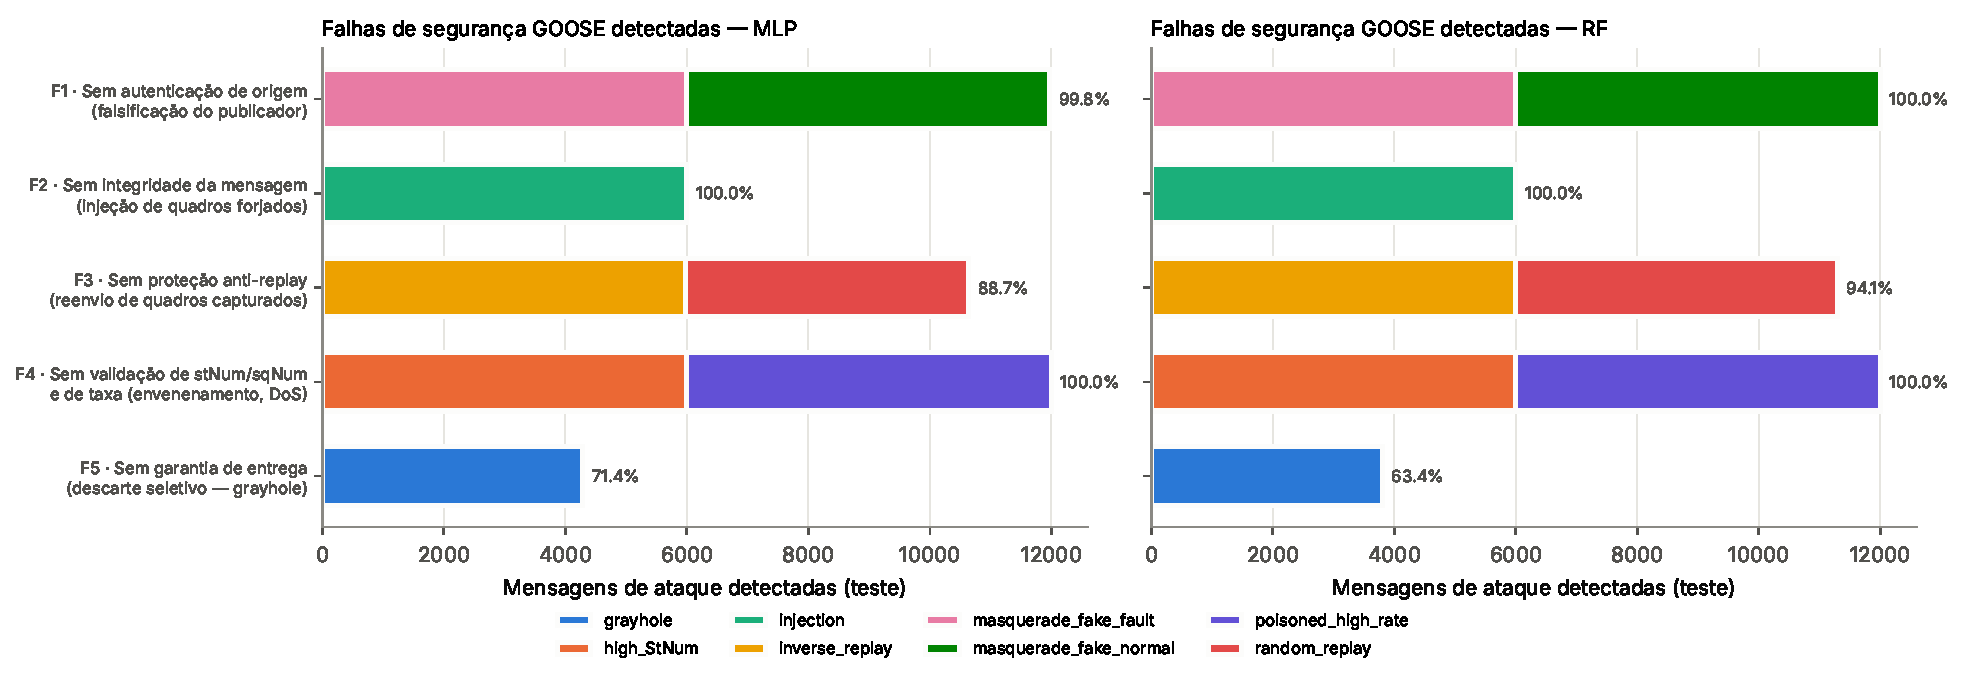
\includegraphics[width=\linewidth]{figuras/fig06_falhas_goose.pdf}
\caption{Mensagens de ataque detectadas por falha de segurança do GOOSE; o
percentual indica a cobertura da falha no teste.}
\label{fig:falhas}
\end{figure}

\subsection{Importância dos atributos}

A Figura~\ref{fig:imp} mostra os 15 atributos mais relevantes para o RF. Os
quatro primeiros são \texttt{timeFromLastChange} (15,7\%), \texttt{StNum}
(15,4\%), \texttt{timestampDiff} (9,7\%) e \texttt{SqNum} (9,1\%), seguidos
por \texttt{confRev} (7,6\%), \texttt{stDiff} (6,9\%) e \texttt{cbStatus}
(6,0\%). Os atributos de cabeçalho e derivados somam a maior parte da
importância; as medidas elétricas contribuem individualmente com menos de
2,2\%. Ainda assim, elas contam: uma ablação com o RF na mesma divisão (§10.1 do
\textit{notebook}) mostra que, só com os 19 atributos de cabeçalho e derivados,
o F1-macro cai de 93,49\% para 91,36\% e o FPR sobe de 13,11\% para 16,37\%. A
perda se concentra no \ataque{random\_replay} (F1 de 92,36\% para 81,50\%) e na
classe \textit{normal} (82,33\% para 77,39\%): o estado elétrico do barramento
ajuda a reconhecer um quadro antigo reenviado fora de contexto. Um detector
restrito aos campos do protocolo, como o de um \textit{switch}, perde essa pista.
A Tabela~\ref{tab:abl} detalha a ablação. Nas demais classes, a diferença é
pequena; \ataque{masquerade\_fake\_fault} perde 2,8 pontos de F1 e
\ataque{grayhole} praticamente não muda, o que confirma que nem os campos do
protocolo nem as medidas elétricas de uma mensagem isolada capturam o descarte
seletivo.

\begin{table}[!htbp]
\centering
\caption{Ablação de atributos no Random Forest (mesma divisão treino/teste), em \%.}
\label{tab:abl}
\small
\begin{tabular}{lcc}
\toprule
Métrica & Protocolo (19 atributos) & Protocolo + elétricos (37)\\
\midrule
Acurácia (9 classes)            & 89,96 & \textbf{92,41}\\
F1-macro                        & 91,36 & \textbf{93,49}\\
TPR (normal $\times$ ataque)    & 91,88 & \textbf{93,95}\\
FPR (normal $\times$ ataque)    & 16,37 & \textbf{13,11}\\
\midrule
F1 \textit{normal}                 & 77,39 & \textbf{82,33}\\
F1 \ataque{grayhole}               & \textbf{67,57} & 67,27\\
F1 \ataque{random\_replay}         & 81,50 & \textbf{92,36}\\
F1 \ataque{masquerade\_fake\_fault}& 97,16 & \textbf{99,96}\\
F1 \ataque{masquerade\_fake\_normal}& 98,90 & \textbf{99,81}\\
\bottomrule
\end{tabular}
\end{table}

\begin{figure}[!htbp]
\centering
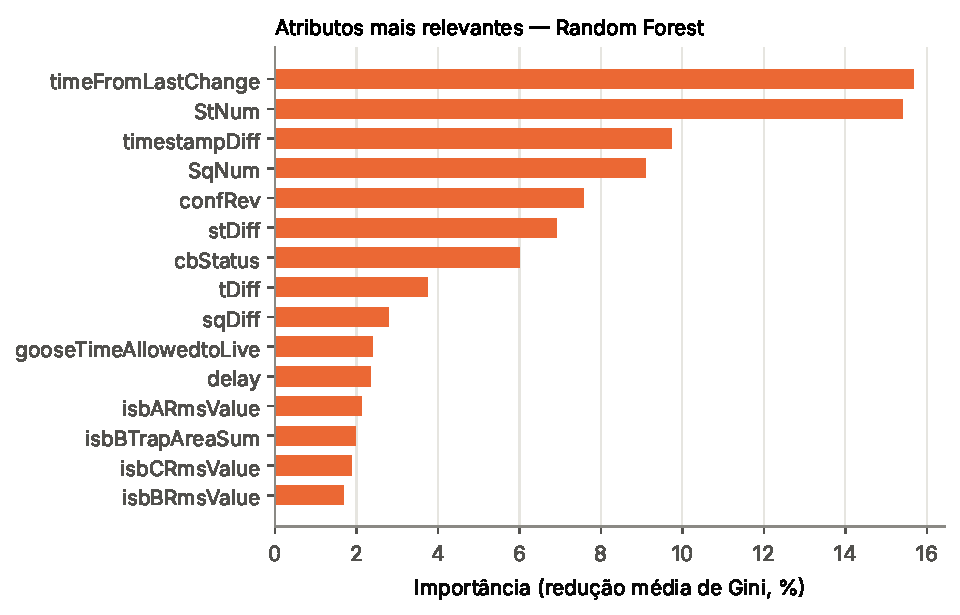
\includegraphics[width=0.5\linewidth]{figuras/fig09_importancia_rf.pdf}
\caption{Atributos mais relevantes para o Random Forest.}
\label{fig:imp}
\end{figure}

\subsection{Fusão com as regras geradas por LLM}

As 22 regras do SBRC~2026 foram aplicadas às mesmas 60.000 mensagens de teste.
Isoladas, alcançam TPR de 32,58\%, FPR de 5,01\% e precisão de 96,30\%
(Tabela~\ref{tab:hib}). A cobertura é desigual: as regras detectam 92,38\% do
\ataque{high\_StNum} e 93,03\% do \ataque{poisoned\_high\_rate}, mas menos de
6\% de \ataque{grayhole}, \ataque{masquerade\_fake\_fault} e
\ataque{random\_replay}. Os falsos positivos vêm, sobretudo, de três regras de
\ataque{grayhole} que testam \texttt{SqNum} baixo, condição frequente também no
tráfego legítimo logo após uma mudança de estado.

A fusão OU com todas as regras aumenta a detecção em apenas 0,12 ponto no RF e
0,13 no MLP, mas eleva o FPR em 4,79 e 4,69 pontos. Com a seleção pelo treino
($\tau=0{,}5\%$), 16 das 22 regras são mantidas: saem as três regras de
\ataque{grayhole} citadas e três regras que não disparam em nenhuma mensagem de
ataque do treino. As regras selecionadas têm FPR de 1,26\% no teste, e o híbrido
seletivo preserva praticamente todo o ganho de detecção da fusão completa com
cerca de um quarto do custo em falsos positivos (+1,15 ponto no RF e +1,09 no MLP). O custo
de avaliar as regras em Python puro é de 2,7~$\mu$s por mensagem.

\begin{table}[!htbp]
\centering
\caption{Visão binária: módulo de assinatura, módulo de anomalia e fusões (\%).}
\label{tab:hib}
\small
\begin{tabular}{lcccc}
\toprule
Configuração & TPR & FPR & Precisão & F1\\
\midrule
Regras LLM (todas, 22)            & 32,58 & 5,01  & 96,30 & 48,69\\
Regras LLM (selecionadas, 16)     & 29,57 & 1,26  & 98,95 & 45,53\\
\midrule
MLP                               & 93,53 & 16,12 & 95,87 & 94,68\\
Híbrido OU (MLP + 22 regras)      & 93,66 & 20,81 & 94,74 & 94,20\\
Híbrido seletivo (MLP + 16 regras)& 93,63 & 17,21 & 95,61 & 94,61\\
\midrule
RF                                & 93,95 & 13,11 & 96,63 & 95,27\\
Híbrido OU (RF + 22 regras)       & 94,07 & 17,90 & 95,46 & 94,76\\
Híbrido seletivo (RF + 16 regras) & 94,04 & 14,26 & 96,35 & 95,18\\
\bottomrule
\end{tabular}
\end{table}

\begin{figure}[!htbp]
\centering
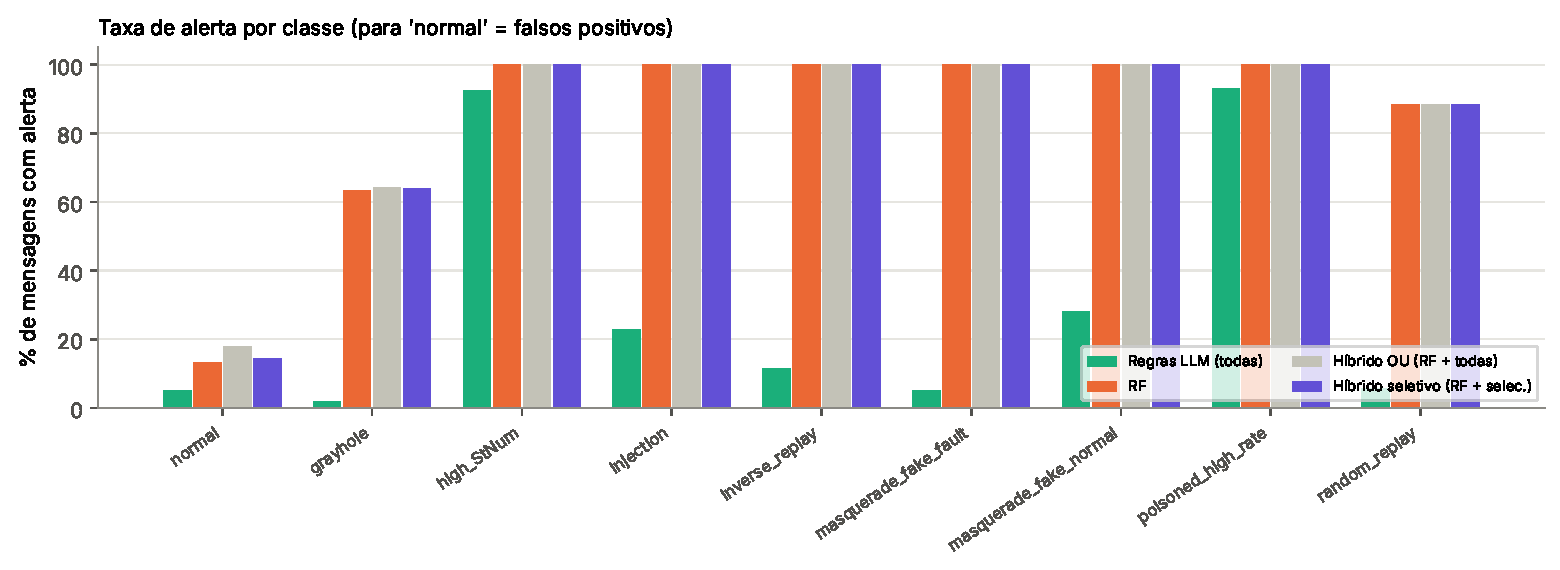
\includegraphics[width=0.92\linewidth]{figuras/fig10_hibrido_por_classe.pdf}
\caption{Taxa de alerta por classe para as regras, o RF e as fusões. Para a
classe \textit{normal}, a taxa corresponde aos falsos positivos.}
\label{fig:hib}
\end{figure}

A Figura~\ref{fig:hib} mostra o efeito por classe. As regras quase não
acrescentam detecção porque o RF já cobre os ataques em que elas são fortes. A
análise dos disparos revela ainda um desalinhamento semântico: várias regras
disparam em ataques diferentes daquele que nomeiam. Por exemplo, a regra
\texttt{rule\_masquerade\_fake\_normal\_stnum\_stdiff} dispara em 5.463
mensagens de \ataque{high\_StNum} e em 1.455 de \ataque{masquerade\_fake\_normal},
e \texttt{rule\_random\_replay\_c} dispara quase só em
\ataque{poisoned\_high\_rate}. As regras são boas detectoras de \emph{ataque},
mas pouco confiáveis para \emph{atribuir} o ataque, papel que cabe ao
classificador.

% =====================================================================
\section{Discussão}\label{sec:disc}

\textbf{Qual modelo usar no módulo de anomalia?} O RF é o mais preciso e o que
gera menos falsos positivos, enquanto o MLP é o único que, na implementação
avaliada, cumpre com folga o limite de 4~ms por mensagem. A escolha depende de
onde o módulo é implantado. Em um IDS fora de banda, alimentado por
espelhamento e com predições em microlotes, o custo por mensagem do RF (8,7~$\mu$s)
é aceitável e sua qualidade justifica a escolha. Em um cenário de decisão
mensagem a mensagem, como uma função de prevenção que bloqueie quadros, o MLP é
mais adequado. Implementações compiladas de florestas e a redução do número de
árvores podem diminuir a latência do RF.

\textbf{Por que \ataque{grayhole} e \ataque{random\_replay} são difíceis?}
Porque os dois ataques não alteram o conteúdo das mensagens que chegam. No
\ataque{grayhole}, as mensagens entregues são legítimas; a evidência está nas
mensagens que \emph{faltam}, ou seja, em saltos de \texttt{sqNum} e em
intervalos maiores que o esperado entre mensagens consecutivas. No
\ataque{random\_replay}, o quadro reenviado é uma cópia válida de um quadro
anterior. Um classificador que olha uma mensagem por vez, com atributos
derivados apenas da mensagem imediatamente anterior, tem acesso limitado a esse
contexto. Isso explica por que as falhas F3 e F5 permanecem abertas e aponta
para atributos de janela (taxa de mensagens por publicador, distribuição dos
saltos de \texttt{sqNum}, número de mensagens esperadas e recebidas por
\texttt{timeAllowedtoLive}) e para modelos sequenciais, como os avaliados por
Moore~\cite{moore2026anomaly}.

\textbf{O que as regras acrescentam ao IDS híbrido?} Neste \textit{dataset}, pouco em
taxa de detecção. O seu valor está em outras propriedades: cada alerta de regra
é explicável pela \textit{red flag} que o originou; o custo é de microssegundos
mesmo em Python; e as regras podem ser executadas no plano de dados, na taxa de
linha. Isso sugere um arranjo em \textbf{cascata}, em que as regras
selecionadas, de alta precisão (98,95\%), bloqueiam no \textit{switch} os ataques
conhecidos, e apenas o tráfego não decidido é encaminhado ao modelo. Como as 16
regras selecionadas já sinalizam cerca de 30\% do tráfego de ataque, a cascata
reduziria a carga do módulo de anomalia sem perda de detecção. Além disso, o
resultado da fusão mostra que regras geradas por LLM precisam de uma etapa de
validação antes da implantação: três das 22 regras eram responsáveis pela maior
parte dos falsos positivos, e a seleção pelo treino é um critério simples e
objetivo para filtrá-las.

\textbf{Onde extrair os atributos?} A ablação da Tabela~\ref{tab:abl} tem uma
consequência direta para a arquitetura. As regras e um classificador embarcado
no \textit{switch} enxergam apenas os campos do protocolo, e com eles o FPR do RF
sobe 3,26 pontos e o F1 do \ataque{random\_replay} cai 10,86 pontos. O módulo de
anomalia deve, portanto, ficar em um ponto da rede com acesso às medidas
elétricas, como um IDS fora de banda que correlacione o tráfego GOOSE com os
valores amostrados do barramento, enquanto o plano de dados fica com as regras.
Essa divisão de papéis reforça o arranjo em cascata discutido acima.

\textbf{Ameaças à validade.} (i) O ERENO é sintético; embora modele a norma com
fidelidade, o desempenho em tráfego real de subestação pode ser diferente,
como Moore observou em avaliação entre ambientes~\cite{moore2026anomaly}.
(ii) A divisão aleatória por mensagem coloca no treino e no teste mensagens
vizinhas no tempo, o que tende a favorecer os modelos; uma divisão por
blocos temporais ou por cenário é mais conservadora. (iii) As regras do
SBRC~2026 foram geradas com base em médias de um subconjunto do mesmo \textit{dataset},
de modo que a comparação não mede a capacidade das regras em ataques novos.
(iv) Não houve busca de hiperparâmetros; os valores reportados são uma linha de
base. (v) As latências foram medidas em um contêiner compartilhado de 2 vCPUs. (vi) Os modelos são
supervisionados e, portanto, só reconhecem como ataque os padrões vistos no
treino; a avaliação com ataques deixados de fora do treino é necessária para
medir a capacidade de detectar ataques desconhecidos.

% =====================================================================
\section{Conclusão e Trabalhos Futuros}\label{sec:conc}

Este artigo construiu o módulo de anomalia de um IDS híbrido para o protocolo
GOOSE e uma ferramenta reprodutível para treiná-lo e avaliá-lo, na qual o
usuário escolhe a base de dados e o algoritmo. No ERENO, o Random Forest foi o
modelo mais preciso, com 92,41\% de acurácia, 93,49\% de F1-macro e 13,11\% de
falsos positivos, e o MLP foi o mais rápido, com 0,20~ms por mensagem, dentro do
limite de 4~ms. Os dois modelos cobrem mais de 99,7\% dos ataques que exploram a
falta de autenticação de origem, de integridade e de validação dos contadores
de estado do GOOSE. A falta de garantia de entrega e de proteção
anti-\textit{replay} continua sendo a fronteira, porque depende de contexto entre
mensagens. A combinação com as regras geradas por LLM no SBRC~2026 mostrou que
uma fusão ingênua aumenta os falsos positivos sem ganho de detecção e que a
seleção das regras pelo treino resolve esse problema.

Como trabalhos futuros, propomos: (i) atributos de janela temporal e modelos
sequenciais (LSTM, GRU) para \ataque{grayhole} e \textit{replay}; (ii) a
avaliação com ataques deixados de fora do treino e com divisão temporal; (iii) a
implementação do arranjo em cascata, com as regras selecionadas no Intel Tofino
e o modelo fora de banda; (iv) a realimentação do \textit{pipeline} LLM com os
erros do modelo, para gerar regras que cubram justamente as lacunas F3 e F5; e
(v) a validação em tráfego de bancada com IEDs reais.

\bibliographystyle{sbc}
\bibliography{referencias}

\end{document}
